\documentclass[aspectratio=169,11pt]{ctexbeamer}
\usetheme{default}
\setbeamertemplate{navigation symbols}{}
\usepackage{graphicx}
\usepackage{booktabs}
\usepackage{hyperref}
\usepackage{xcolor}

\definecolor{main}{RGB}{20,83,74}
\definecolor{accent}{RGB}{191,138,38}
\definecolor{textgray}{RGB}{55,64,72}
\definecolor{light}{RGB}{240,246,243}

\setbeamercolor{background canvas}{bg=white}
\setbeamercolor{normal text}{fg=textgray,bg=white}
\setbeamercolor{frametitle}{fg=white,bg=main}
\setbeamercolor{title}{fg=main}
\setbeamercolor{block title}{fg=main,bg=light}
\setbeamercolor{block body}{fg=textgray,bg=white}
\setbeamercolor{item}{fg=main}
\setbeamertemplate{frametitle}{
  \nointerlineskip
  \begin{beamercolorbox}[wd=\paperwidth,ht=3.6ex,dp=1.2ex,leftskip=0.8cm]{frametitle}
  \insertframetitle
  \end{beamercolorbox}
}
\setbeamertemplate{footline}{
  \leavevmode\hbox{\begin{beamercolorbox}[wd=.82\paperwidth,ht=2.8ex,dp=1ex,leftskip=.5cm]{author in head/foot}\scriptsize 气候政策多利益相关方博弈沙盘原版项目\end{beamercolorbox}\begin{beamercolorbox}[wd=.18\paperwidth,ht=2.8ex,dp=1ex,rightskip=.5cm,right]{date in head/foot}\scriptsize \insertframenumber/\inserttotalframenumber\end{beamercolorbox}}
}

\title{气候政策多利益相关方博弈沙盘}
\subtitle{原版项目课堂汇报 PPT}
\author{课程大作业展示}
\date{\today}

\begin{document}

\begin{frame}[plain]
  \vspace{1.2cm}
  {\Huge\color{main}\bfseries 气候政策多利益相关方博弈沙盘}\par
  \vspace{0.4cm}
  {\Large\color{textgray}基于规则引擎与 AI 叙事增强的课堂原型}\par
  \vspace{0.8cm}
  \begin{itemize}
    \item 研究问题：气候政策如何在多方约束下达成可接受妥协
    \item AI 作用：辅助建模、编码、叙事生成与结果整理
    \item 输出成果：可运行原型、历史回放、技术报告、展示材料
  \end{itemize}
  \vfill
  {\small \color{accent}建议讲法：开场 20 秒直接说“我们做的不是聊天机器人，而是一个气候政策协商沙盘”。}
\end{frame}

\begin{frame}{1. 研究问题为什么重要}
\begin{itemize}
  \item 气候政策不是单一减排目标，而是\textbf{减排、公平、融资、能源安全、产业转型}的综合平衡。
  \item 课堂辩论通常只能展示一次立场碰撞，难以重复、难以比较、难以回放。
  \item 我们的问题是：\textbf{给定一条政策提案，不同利益相关方会如何回应，阻力来自哪里，怎样才能谈成最低可接受妥协？}
\end{itemize}
\begin{block}{项目定位}
不是做真实世界预测系统，而是做一个低成本、可解释、适合教学展示的政策协商原型。
\end{block}
\end{frame}

\begin{frame}{2. AI 是怎么帮助我们完成项目的}
\begin{columns}[T]
\column{0.5\linewidth}
\begin{itemize}
  \item 用 AI 辅助收敛研究问题，明确范围
  \item 用 AI 整理典型角色与谈判诉求
  \item 用 AI 提升编码效率与界面实现速度
\end{itemize}
\column{0.5\linewidth}
\begin{itemize}
  \item 用规则引擎保证结果稳定和可解释
  \item 用大模型把结构化立场转成自然发言
  \item 用 AI 生成图表、报告和汇报材料
\end{itemize}
\end{columns}
\begin{alertblock}{一句话总结}
AI 在这个项目里不是“替我们决定答案”，而是帮助我们更快完成建模、开发、表达和展示。
\end{alertblock}
\end{frame}

\begin{frame}{3. 系统怎么工作}
\centering
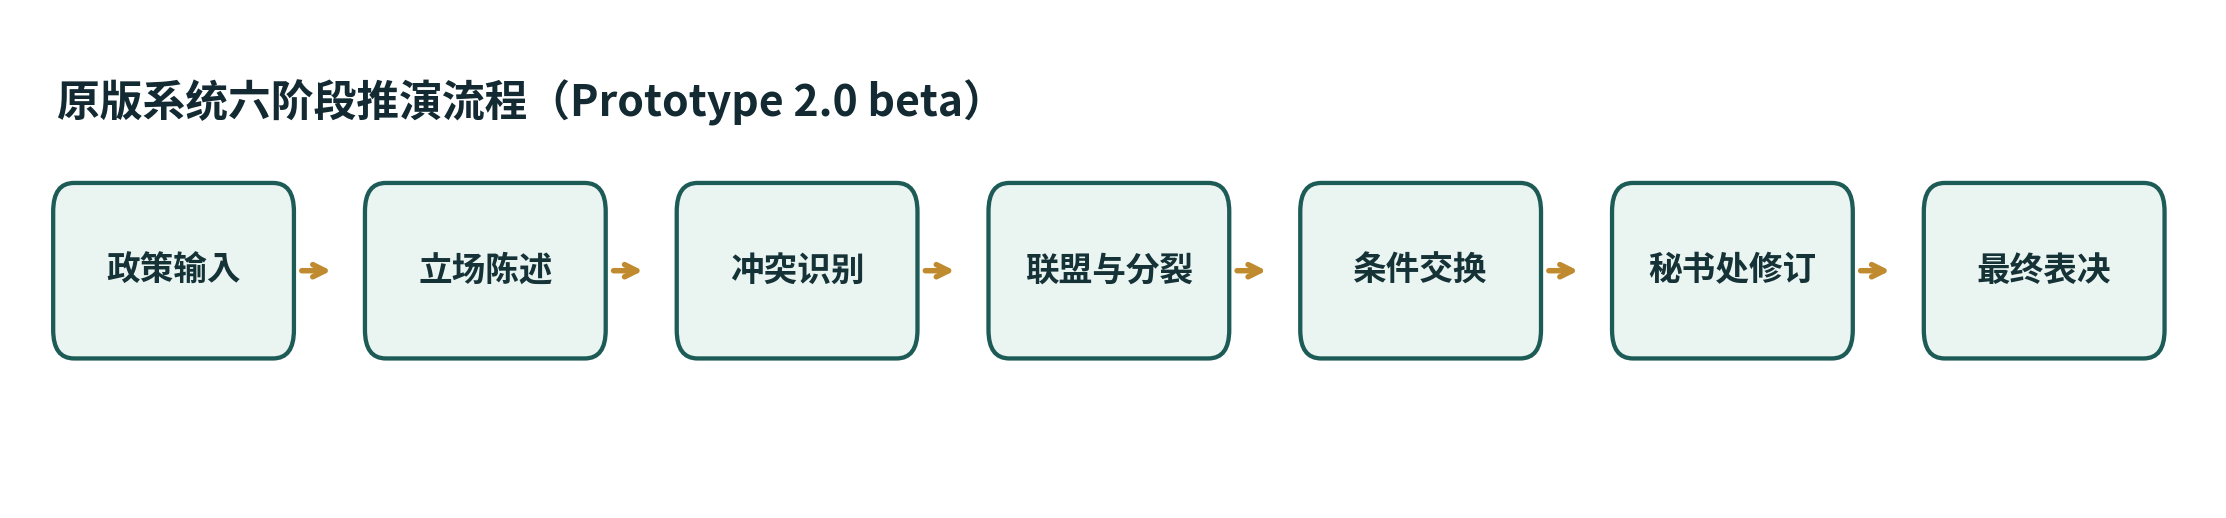
\includegraphics[width=0.96\textwidth]{../figures/pipeline_overview.png}
\vspace{0.4cm}
\begin{itemize}
  \item 输入一条政策文本，先抽取为结构化政策维度
  \item 让不同角色基于权重、诉求和约束生成立场
  \item 再识别冲突、联盟、交换条件和修订结果
\end{itemize}
\end{frame}

\begin{frame}{4. 为什么这个原型是可解释的}
\begin{itemize}
  \item 当前原版不是完全自由对话，而是\textbf{规则驱动的多角色协商引擎}
  \item 每个角色都有清晰身份配置：描述、设计依据、优先诉求、偏好权重
  \item 系统支持两种模式：
  \begin{itemize}
    \item 抽象角色模式：更适合解释谈判结构
    \item 真实国家样本模式：更适合展示真实性与可追溯性
  \end{itemize}
  \item 每次运行都能保存本地历史记录，支持回放与复现实验
\end{itemize}
\begin{block}{当前边界}
这是“有现实约束的规则推演”，不是 IAM，也不是完全自治的多智能体系统。
\end{block}
\end{frame}

\begin{frame}{5. 实验结果一：不同运行样本的核心指标}
\centering
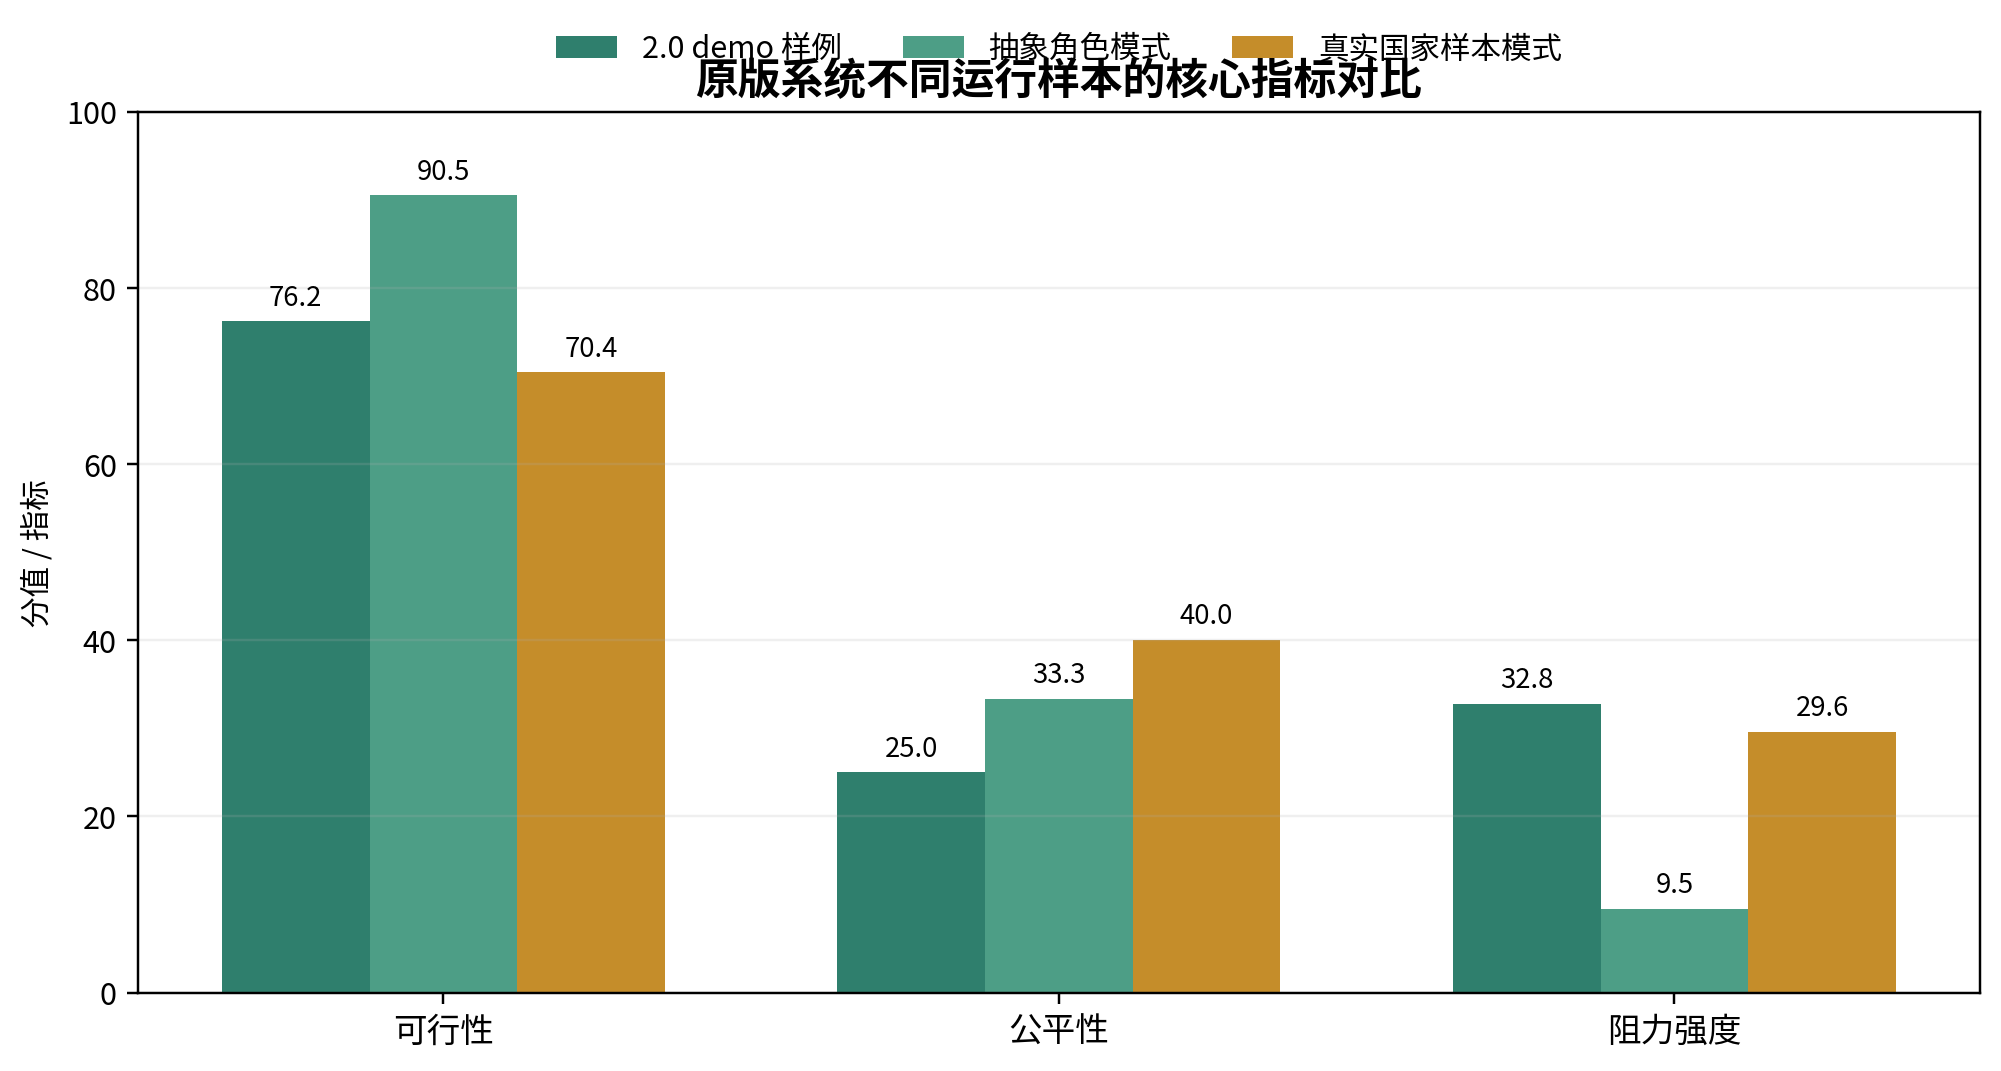
\includegraphics[width=0.88\textwidth]{../figures/metrics_comparison.png}
\vspace{0.2cm}
\begin{itemize}
  \item 高冲突政策会显著拉高阻力强度
  \item 更平衡的政策更容易在抽象角色模式下形成较强共识
  \item 真实国家样本模式会引入更多现实摩擦，因此结果更“保守”
\end{itemize}
\end{frame}

\begin{frame}{6. 实验结果二：谁在支持，谁在反对}
\begin{columns}[T]
\column{0.52\linewidth}
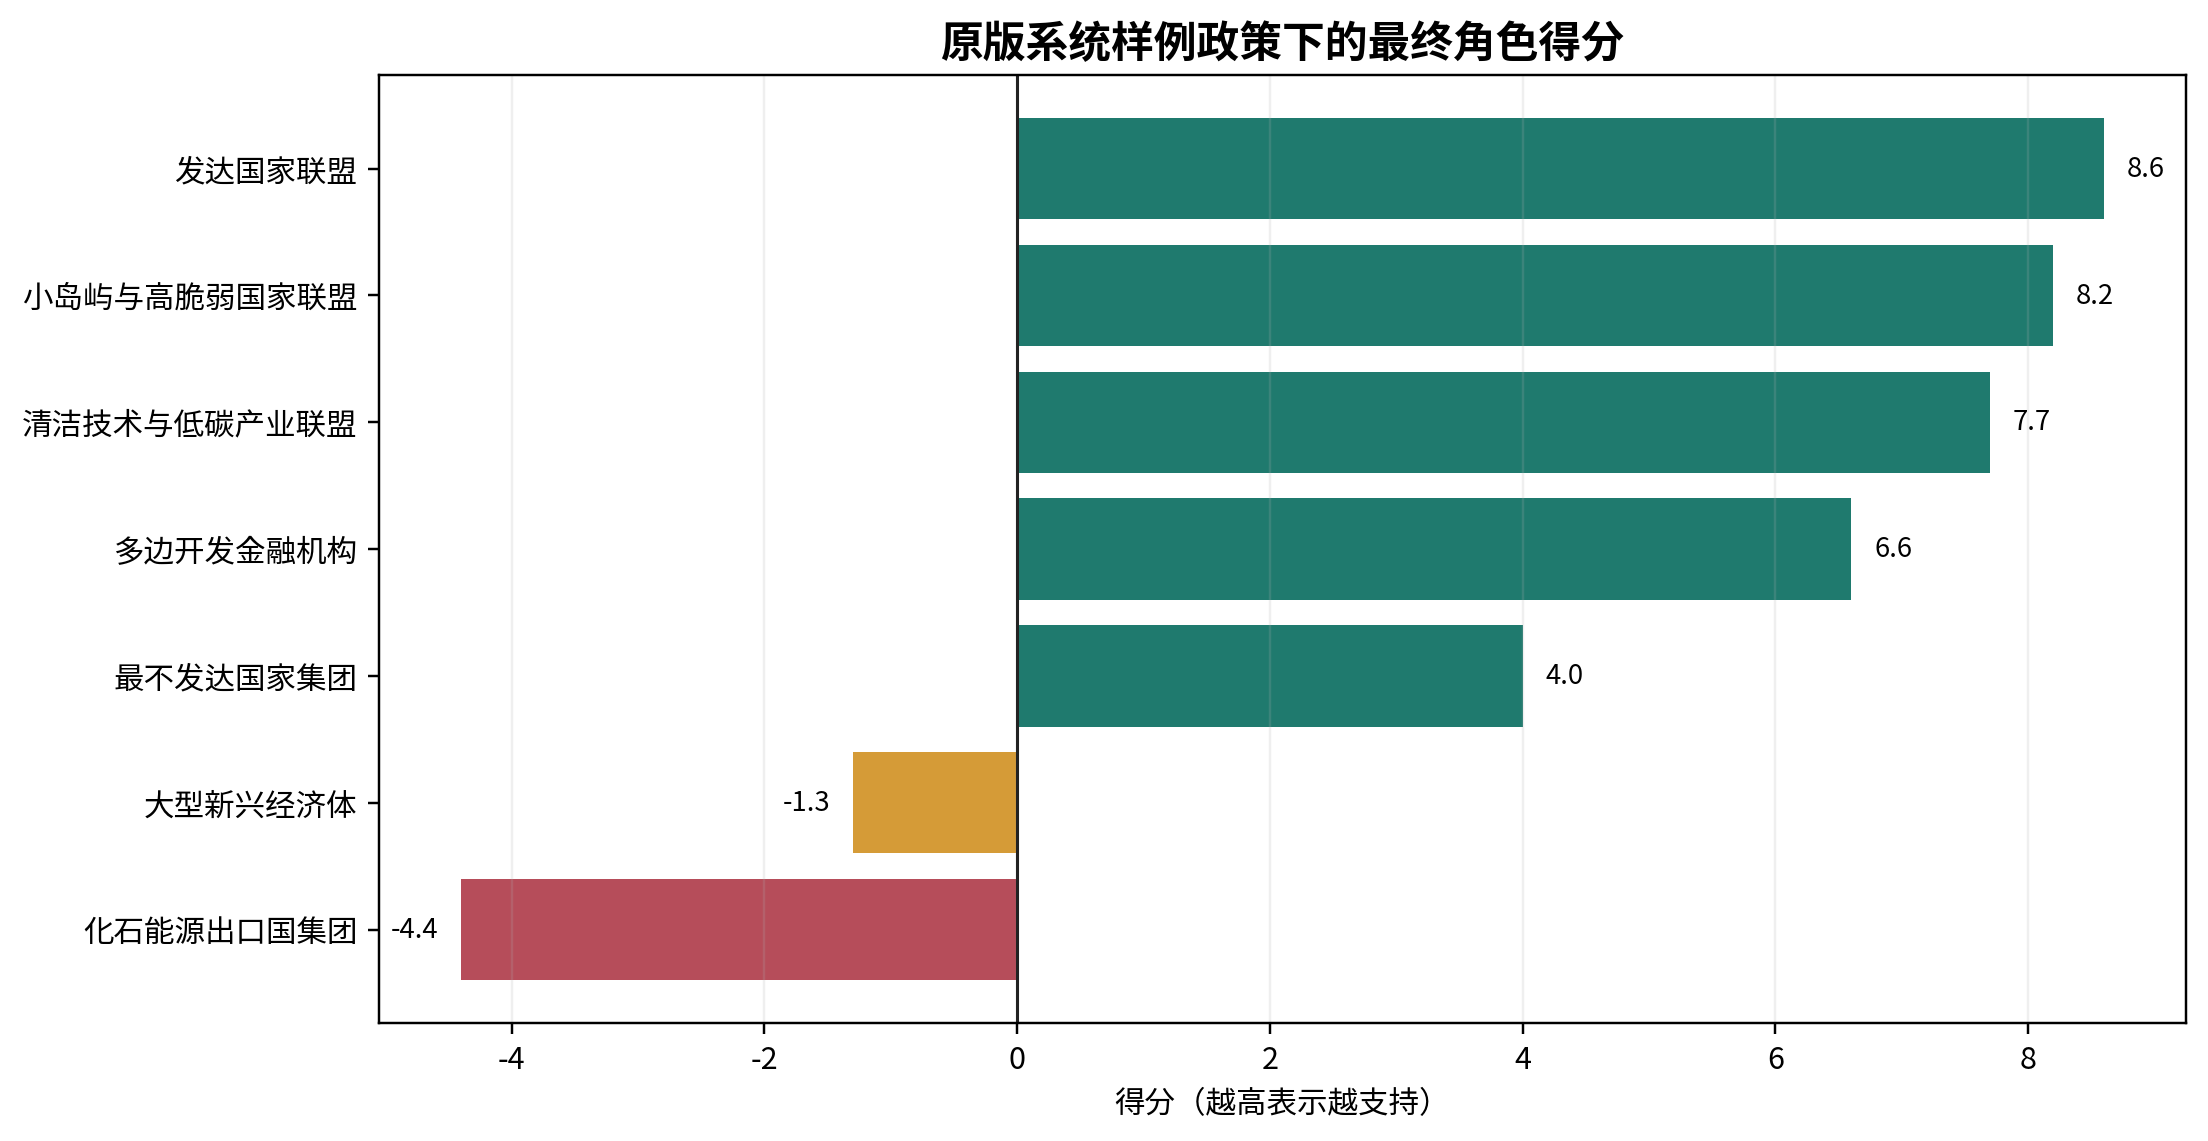
\includegraphics[width=\linewidth]{../figures/agent_scores_demo.png}
\column{0.44\linewidth}
\begin{itemize}
  \item 发达国家联盟、清洁技术联盟、小岛屿联盟总体支持
  \item 化石能源出口国和大型新兴经济体对高强度退出更敏感
  \item 系统给出的不是一句抽象判断，而是具体的支持/反对分布
\end{itemize}
\end{columns}
\end{frame}

\begin{frame}{7. 实验结果三：系统如何给出妥协路径}
\begin{columns}[T]
\column{0.58\linewidth}
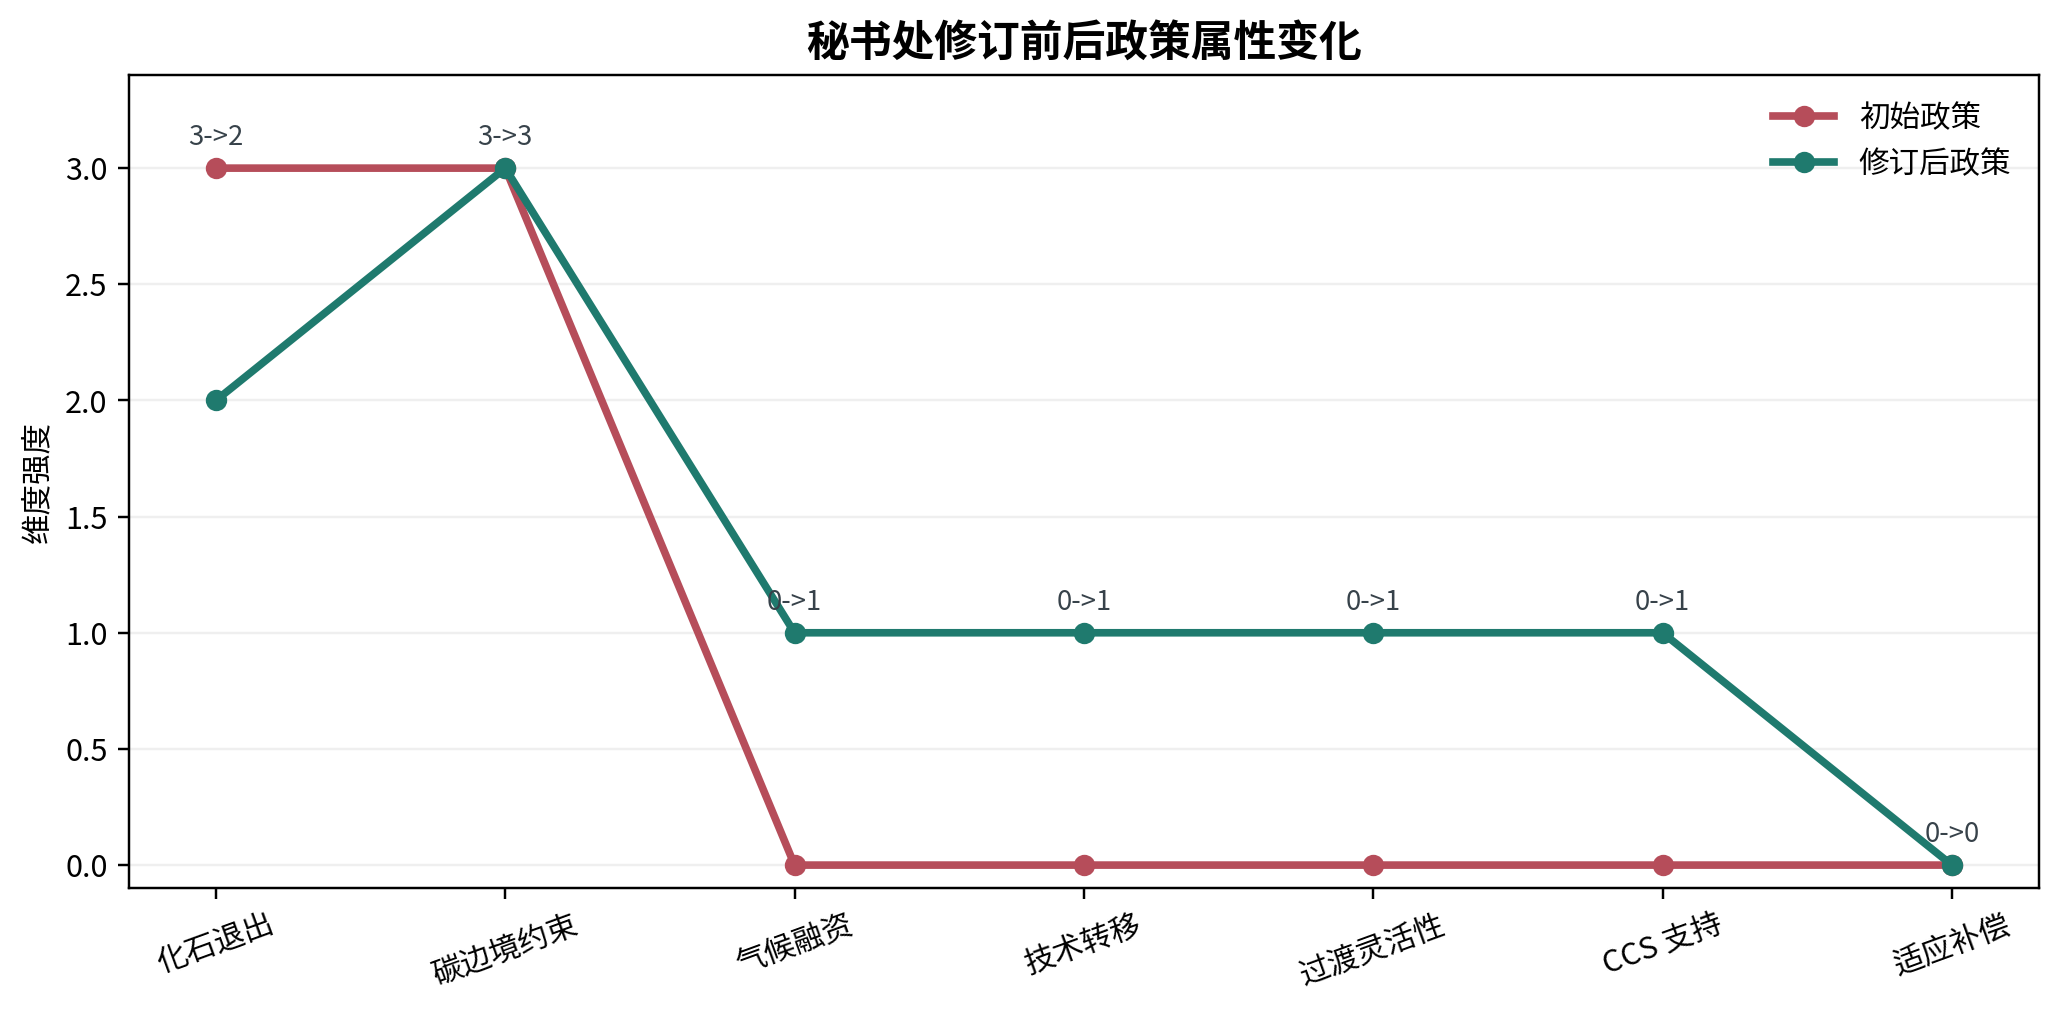
\includegraphics[width=\linewidth]{../figures/policy_adjustments.png}
\column{0.38\linewidth}
\begin{itemize}
  \item 初始政策：强退出 + 强边境约束
  \item 系统识别核心冲突后，自动建议：
  \begin{itemize}
    \item 弱化退出强度
    \item 增加融资与技术转移
    \item 增加过渡期和 CCS 支持
  \end{itemize}
  \item 这就是“从冲突到妥协”的关键价值
\end{itemize}
\end{columns}
\end{frame}

\begin{frame}{8. 结论与答辩重点}
\begin{block}{主要结论}
\begin{itemize}
  \item 气候政策可行性高度依赖融资、技术、过渡与公平安排
  \item 纯高压减排要求会迅速激化多方冲突
  \item 规则引擎 + AI 叙事是一条适合课堂项目的高性价比路线
\end{itemize}
\end{block}
\begin{alertblock}{答辩时重点讲清楚}
\begin{itemize}
  \item 研究问题的意义：为什么气候政策天然是多方博弈
  \item AI 辅助流程：AI 如何帮助我们更快完成建模与表达
  \item 主要结论：什么样的政策更容易谈成，阻力主要来自谁
\end{itemize}
\end{alertblock}
\vfill
{\small 如果老师追问局限，可以直接回答：当前版本更偏规则驱动原型，下一步会向真正多 agent 协商系统升级。}
\end{frame}

\end{document}
